% multiple1902 <multiple1902@gmail.com>
% bachelor.tex
% Copyright 2011~2012, multiple1902 (Weisi Dai)
% https://code.google.com/p/xjtuthesis/
% 
% It is strongly recommended that you read documentations located at
%   http://code.google.com/p/xjtuthesis/wiki/Landing?tm=6
% in advance of your compilation if you have not read them before.
%
% This work may be distributed and/or modified under the
% conditions of the LaTeX Project Public License, either version 1.3
% of this license or (at your option) any later version.
% The latest version of this license is in
%   http://www.latex-project.org/lppl.txt
% and version 1.3 or later is part of all distributions of LaTeX
% version 2005/12/01 or later.
%
% This work has the LPPL maintenance status `maintained'.
% 
% The Current Maintainer of this work is Weisi Dai.
%
\documentclass[
    bachelor, 
    %bigskip, % sets linespread factor to 1.5
    truefont, % just turn it on when using Windows
    %nofont, % remember to manally set the fonts
    pdflinks,
    %colorlinks,
    %compact,
    ]{xjtuthesis}

\graphicspath{{figures/}}

% my settings
% 
%\usepackage[numbers,square,super,sort&compress]{natbib} % original bib格式
\usepackage[round,sort&compress]{natbib}
%\bibliographystyle{gbt7714-2005-xjtu}
\bibliographystyle{plainnat}
%\renewcommand{\refname}{References}
%罗马数字
\newcommand{\RNum}[1]{\uppercase\expandafter{\romannumeral #1\relax}}
%写化学式
\usepackage[version=4]{mhchem}
%修改列表环境
\usepackage{enumitem}
%\setenumerate[1]{itemsep=0pt,partopsep=0pt,parsep=\parskip,topsep=5pt,leftmargin=2em}
\setitemize[1]{itemsep=-6pt,partopsep=0pt,parsep=6pt,topsep=5pt}
%\setdescription{itemsep=0pt,partopsep=0pt,parsep=\parskip,topsep=5pt}
%插图
\usepackage{graphicx}
%单元格内强制换行
\newcommand{\tabincell}[2]{\begin{tabular}{@{}#1@{}}#2\end{tabular}}
\renewcommand{\arraystretch}{1.35}%调整矩阵行间距

\begin{document}

    % multiple1902 <multiple1902@gmail.com>
% meta.tex
% Copyright 2011~2012, multiple1902 (Weisi Dai)
% https://code.google.com/p/xjtuthesis/
% 
% It is strongly recommended that you read documentations located at
%   http://code.google.com/p/xjtuthesis/wiki/Landing?tm=6
% in advance of your compilation if you have not read them before.
%
% This work may be distributed and/or modified under the
% conditions of the LaTeX Project Public License, either version 1.3
% of this license or (at your option) any later version.
% The latest version of this license is in
%   http://www.latex-project.org/lppl.txt
% and version 1.3 or later is part of all distributions of LaTeX
% version 2005/12/01 or later.
%
% This work has the LPPL maintenance status `maintained'.
% 
% The Current Maintainer of this work is Weisi Dai.
%
\ctitle{蛋清中溶菌酶的分离提取和性质实验}
\cauthor{高旭帆,郭骐瑞,程肖然,黎博琛}
\csubject{生命科学综合实验\Rnum{1}}
\csupervisor{孔宇,李华}
\ckeywords{溶菌酶;分离提取;阳离子交换色谱;SDS-PAGE}
\cproddate{\the\year 年\the\month 月}
\ctype{实验研究}

\etitle{Separation and Extraction of Lysozyme from Egg White and Characterization}
\eauthor{Xufan Gao, Qirui Guo, Xiaoran Cheng, Bochen Li}
\esupervisor{Yu Kong, Hua Li}
\ekeywords{Lysozyme; Separation and Extraction; Cation exchange chromatography; SDS-PAGE}
\ecate{Biology}
\esubject{Integrated Experiments of Life Sciences \Rnum{1}}
\eproddate{\monthname{\month}\ \the\year}
\etype{Experimental Research}

\cabstract{
溶菌酶是一种能水解N-­乙酰胞壁酸 (NAM)和N­-乙酰氨基葡萄糖之间的 β­-1,4糖苷键,从而破坏细菌细胞壁的酶,目前已广泛应用于食品、医疗、生物等产业。但是这种天然产物的分离纯化方法还有待完善。本研究从蛋清中提取溶菌酶,用阳离子交换和凝胶层析的方法进行纯化,并测定溶菌酶浓度和检测其抗菌活性。最终通过对SDS-PAGE实验结果进行比较分析,发现阳离子交换的方法可以达到更好的纯化效果,使样品中基本上不含杂蛋白。纯化得到的样品的比活力达到13\emph{.}4,回收率达到非常可观的92\emph{.}4\%。最后,通过探究不同方程对于数据的拟合,发现并解释了函数\(f(t)=at^2 + bt + c\)在拟合时更好的表现。经过提取纯化后的溶菌酶结合可控释放和酶固定化的技术将在食品储存和医疗保健领域得到应用。
%向那些疯狂的家伙们致敬, 
%他们特立独行, 
%他们桀骜不训, 
%他们惹是生非, 
%他们格格不入.
%
%他们用与众不同的眼光看待事物, 
%他们不喜欢墨守成规, 
%他们也不愿安于现状.
%
%你可以赞美他们, 引用他们, 反对他们, 
%质疑他们, 颂扬或是诋毁他们, 
%但唯独不能漠视他们. 
%
%因为他们改变了事物. 
%他们推动人类向前发展. 
%
%或许他们是别人眼里的疯子, 
%但却是我们眼中的天才. 
%
%因为只有那些疯狂到以为自己能够改变世界的人, 
%才能真正地改变世界. 
}

\eabstract{
Lysozyme is a kind of enzyme that can hydrolyze the β-1,4 glycosidic
bond between N-acetyl muramic acid (NAM) and N-acetyl glucosamine, thus
destroy the bacterial cell wall. Nowadays, they have been widely applied
to food, medical, and biological industries. However, the separation and
purification methods still need perfection for this natural product. In
this work, lysozyme was extracted from egg white and purified by cation exchange and gel chromatography. Its concentration was determined and
its antibacterial activity was tested. Finally, through the comparative
analysis of SDS-PAGE experimental results, it is found that cation exchange can achieve a better purification effect so that the
sample basically does not contain other proteins. The specific activity
of the sample purified reached \(13.4\mathrm{U\cdot mg^{ - 1}}\), and
the recovery rate reached \(92 .  4\%\). Finally, by exploring the
fitting of different equations to the data, it is found and explained
that the function \(f(t)= at ^ 2 +  bt  +  c \) performs best in the
fitting. The purified lysozyme combined with controlled release and
enzyme immobilization technology will be applied in the field of food
storage and health care.

%Here's to the crazy ones. The misfits. The rebels. The troublemakers. The round pegs in the square holes. 
%
%The ones who see things differently. They're not fond of rules. And they have no respect for the status quo. You can quote them, disagree with them, glorify or vilify them. 
%
%About the only thing you can't do is ignore them. Because they change things. They push the human race forward. 
%
%While some may see them as the crazy ones, we see genius. Because the people who are crazy enough to think they can change the world, are the ones who do.
%
%(Apple Inc.)

}


    \xjtucinfopage
    \xjtueinfopage
    \xjtutoc
    \clearpage

%    % multiple1902 <multiple1902@gmail.com>
% denotation.tex
% Copyright 2011~2012, multiple1902 (Weisi Dai)
% https://code.google.com/p/xjtuthesis/
% 
% It is strongly recommended that you read documentations located at
%   http://code.google.com/p/xjtuthesis/wiki/Landing?tm=6
% in advance of your compilation if you have not read them before.
%
% This work may be distributed and/or modified under the
% conditions of the LaTeX Project Public License, either version 1.3
% of this license or (at your option) any later version.
% The latest version of this license is in
%   http://www.latex-project.org/lppl.txt
% and version 1.3 or later is part of all distributions of LaTeX
% version 2005/12/01 or later.
%
% This work has the LPPL maintenance status `maintained'.
% 
% The Current Maintainer of this work is Weisi Dai.
%
\begin{denotation}

  \item[\xjtuthesis]    我能吞下玻璃而不伤身体噢
  \item[Linux]          李氏操作系统
  \item[Windows]        温氏操作系统

\end{denotation}


    \xjtucontent

        % multiple1902 <multiple1902@gmail.com>
% intro.tex
% Copyright 2011~2012, multiple1902 (Weisi Dai)
% https://code.google.com/p/xjtuthesis/
% 
% It is strongly recommended that you read documentations located at
%   http://code.google.com/p/xjtuthesis/wiki/Landing?tm=6
% in advance of your compilation if you have not read them before.
%
% This work may be distributed and/or modified under the
% conditions of the LaTeX Project Public License, either version 1.3
% of this license or (at your option) any later version.
% The latest version of this license is in
%   http://www.latex-project.org/lppl.txt
% and version 1.3 or later is part of all distributions of LaTeX
% version 2005/12/01 or later.
%
% This work has the LPPL maintenance status `maintained'.
% 
% The Current Maintainer of this work is Weisi Dai.
%
%\chapter{绪论}
%\echapter{Preface}
\chapter{Preface}

\section{Physicochemical Properties}
Lysozyme (EC 3.2.1.17) is a protein existing in animals, plants, bacteria, and viruses. It can be found in neutrophils, macrophage granules, serum, saliva, milk, honey, and eggs. The enzyme hydrolyzed β-1,4 glycosidic bond between N-acetyl muramic acid (NAM) and N-acetyl glucosamine (NAG) of cytoderm peptidoglycan (PG) in Gram-positive and Gram-negative bacteria \citep{Gajda2014}. C-type lysozyme of egg white is a model for studying protein structure and function. 

\subsection{Structure and Mechanism}

The three-dimensional structure of lysozyme was first resolved in 1965 by X-ray \citep{Blake1965}. Lysozyme consists of 129 amino acids cross-linked by 4 disulfide bonds, and lysozyme has two main domains. The α domain of the molecule is mainly composed of α helix, while the β domain contains β fold and helix. The active site is in the gap between the two domains. 

There are two catalytic mechanisms to explain lysozyme. According to the Phillips mechanism, two residues Glu35 (glutamic acid) and Asp52 (aspartic acid) play an important role. The terminal proton of Glu35 is transferred to the O atom of the glycosidic bond between two adjacent sugar residues, which leads to cleavage of glycosidic bond and formation of a carbocation. The positive charge of the carbocation is stabilized by the negative charge of Asp52 until the hydroxide ion binds to the positive C atom and Glu35 is protonated. Another is Intermediate theory. Like all other retained β-glucosidases, egg white lysozyme proceeds through the formation of covalent intermediates and subsequent decomposition rather than through the formation of long-lived ion pairs \citep{Vocadlo2001}. The latest research supports the Phillips mechanism more \citep{Held2014}.

\begin{figure}[!h]
	\centering
	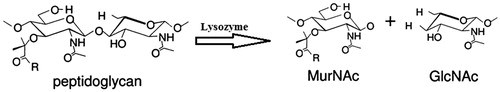
\includegraphics[width=0.9\linewidth]{figures/chp1_lysozyme_mechanism}
	\caption{The Reaction. Extracted from \cite{Ercan2016}}
	\label{fig:chp1lysozymemechanism}
\end{figure}

\subsection{Function and Applications}
Lysozyme has broad-spectrum resistance to both Gram-negative and Gram-positive bacteria. The bactericidal ability of lysozyme is not only due to its catalytic activity but also due to its cationic and hydrophobic characteristics \citep{Pellegrini1992}. Chemical modifications such as oleoyl chloride \citep{Evran2010} and Na2SO3 \citep{Liu2018} can enhance the hydrophobic properties of lysozyme and enhance its antibacterial effect. Research \citep{Ibrahim2001} proved that the helix-loop-helix domain located in the 87–114 sequence of lysozyme and its C-terminal helix domain passed through the outer membrane and damaged the inner membrane through self-promoting absorption, thus killing Gram-negative bacteria. In the human body, lysozyme degrades bacteria not only by directly killing bacteria but also by releasing immune regulatory bacterial ligands including PG fragments to participate in the regulation of the immune system \citep{ragland2017bacterial}. PG fragment can eliminate bacteria by enhancing the activation of phagocytes.

Egg white is composed of lysozyme, accounting for about 0.5\% of its weight. At present, egg white lysozyme occupies a dominant position in the market, and its main limitations are high recovery cost, low activity, and immunological problems \citep{Ercan2016}. This immunological problem is dominated by IgE \citep{Urisu2015}, and people who are allergic to eggs will cause immunological problems, so the production of human lysozyme is also an important research direction. At present, the human lysozyme gene is expressed in heterologous organisms, such as rice \citep{R.Wilken2011} and yeast \citep{Huang2009}. Studies in rice have proved that the manufacturing cost (\$/g) is the same as that of eggs \citep{R.Wilken2011}.



\section{Discussion on the Application}
Given the ability to lyse the cell wall of bacterial,
lysozyme has been attracting immense attention as a kind of 
environment-friendly or organs-friendly antimicrobial.
As we have discussed before, it has nowadays more and more applications in the food industry and clinical procedures. In this part, we will discuss 
it's applications within our preparations and capabilities.

\subsection{Applications in Food Industry}
Our first focus is on the food industry. Since the 1800s when Napoléon launched his strategy to conquer Europe, the storage or preservation of food has become a major question in the food industry. Sealing food in cans, High-temperature treatment, Pasteurization, numerous methods had risen. And in the last, people introduced chemical additives to the food industry. Efficient as it is, nowadays people are having less tolerance in that chemical industry. Due to the conception of eating healthy, they prefer so-called "Non-additive food" to chemical treated food. But the lack of bacterial inhibition will easily make it a perfect bacterial petri dish. The chemical hazard vanishes, but the microbial hazard just arises. We need another method!

So we cast our sight to the biological method to preserve food. In our case, we are planning to introduce lysozyme to food packing and food additives. As for the food packing, we are going to distribute the lysozyme agent, in gluten \citep{Conte2006} or onto a chitosan powder, on the food packages, mostly LDPE, these methods have been taken into practice \citep{Borzooeian2017}. And its function to extend to the shelf life of foods had been proved \citep{Lian2012, Alhazmi2014}. our points of view, this kind of application suits our capability very well, and we have put it into our first consideration.

Another important application in the food industry is the food additive. We can add some lysozyme into specific easy-deteriorating foods, such as wurst, can-foods, and diary. The addition of lysozyme will significantly extend the preserve half-life of food, these lysozymes are presented into chitosan particals \citep{Wu2017}, this will not only protect the original flavour of the food but also enhance its ability to inhibit bacterial emerging.

\subsection{Clinical Applications}
The lysozyme can also play an impressive role in the clinical procedure. Like the food industry, medical is also a battel against bacterial. In 1676, Anton van Leeuwenhoek observed bacteria and other microorganisms, using a single-lens microscope of his design.
In 1796, Edward Jenner developed a method using cowpox to successfully immunize a child against smallpox. The same principles are used for developing vaccines today.
Following on from this, in 1857 Louis Pasteur also designed vaccines against several diseases such as anthrax, fowl cholera and rabies as well as pasteurization for food preservation.
In 1867 Joseph Lister is considered to be the father of antiseptic surgery. By sterilizing the instruments with diluted carbolic acid and using it to clean wounds, post-operative infections were reduced, making surgery safer for patients.
In 1929 Alexander Fleming developed the most commonly used antibiotic substance both at the time and now: penicillin \citep{Brock2003}.The emerge of antibiotic medicine start a new era for human, we can sometimes beat the infection of microbes.

But there still exists a fatal problem: ALLERGY. Some antibiotics will lead to an acute allergic phenomenon, which is sometimes fatal. So we come up with this idea to introduce lysozyme to health-care products. We want to introduce it in for instance dentifrices, mouth-rinses, moisturizing gels, chewing gums or such sterilization products \citep{Tenovuo2002}.
We try to develop a kind of lysozyme covered bandage in which the lysozyme exist in gel, or in other advanced status, such as carbon nanotubes.

These are our prospects of the clinical application of lysozyme.


%应用的原理也说一点。让老师感觉有用(但也就是个大概。老师看了能提意见?

%\section{溶菌酶的应用}
\section{Applications of Lyzoenzymes}
%溶菌酶在食品、医药、生物技术等方面都有广泛的应用
Here we conducted a summary of current research on the application of lysozymes. We find that our two ideas are practical and potentially valuable in our daily life. Today lysozymes have been widely applied to food, medical, and biological industries. 

%\subsection{食品和发酵}
\subsection{Applications in Food and Fermentation Industry}

%我国食品工业生产过程中广泛使用化学合成防腐剂,它们对人体可能有潜在的毒副作用;而溶菌酶就是一种天然防腐剂。
%溶菌酶本身对人体没有毒害作用,缺可以很好地抑制细菌的生长,有效地延长食品的保质期。
Natural lysozymes can repress bacterial growth without undermining our health thus they are mainly used as preservatives. \citet{ZHAI2015} demonstrate in their review that lysozymes can prevent cheese from microorganism-caused swelling during the production; they also have an outstanding effect in retaining the freshness of meat product combined with other natural preservatives.
\citet{Yu-tong2006} and \citet{ZHAI2015} all show that lysozymes are added into Japanese sake (a kind of low wine) to replace salicylic acid or \ce{SO2} in as the preservative. Microorganisms are initiators of aquatic products' rotting. \citet{Ren2013} point out in their review that lysozymes may do better than instant cool storage with the help of some other techniques like ultrahigh pressure.

%\citet{ZHAI2015}在其综述中发现,“溶菌酶和其他天然防腐剂复合而成的保鲜剂,在鲜肉和熟制肉品的保鲜过程中确实有明显的效果”;干酪生产过程中,微生物的发酵会导致干酪的膨胀,而添加溶菌酶能抑制这种微生物的生长。微生物也是引起水产品腐败变质的主要原因,\citet{Ren2013}在其综述中指出,溶菌酶的应用使得某些水产品的保存效果优于冷藏,但需要配合多种溶菌酶或其他保存措施使用

\subsection{Applications in Medical Industry}
Lysozymes are a component of the second line of immune defense in our body for their nonspecific bactericidal effect. Moreover, people are adding extra lysozymes to strengthen our immune system or cure inflammation and infection. Lysozymes can also improve the therapeutic effect of various kinds of drugs. 

According to \cite{Yu-tong2006} and \cite{ZHAI2015}, lysozymes can regulate gut microbes by specifically killing putrefactive ones and selectively increase the number of bifidobacterium, which is a significant intestinal probiotic. Therefore, lysozymes bring remission to enteritis and enhance the immune system. It is pretty helpful for susceptible infants.  Adding lysozyme to milk is widely applied as a quality-improvement strategy.
Lyzozymes extracted from egg white are also made into industralized mouth wash, which can inhibit the growth of over 99\% \textit{Escherichia coli} and \textit{Staphylococcus aureus} \citep{Unknown2020}.
%但溶菌酶也不是要杀灭所有微生物,相反,还具有调节肠道微生物的功能。它对肠道中腐败性微生物有特殊的杀灭作用,却促进双歧杆菌的生长。双歧杆菌是一种重要的肠道有益微生物,为人体提供生物屏障和营养、免疫增强作用。在乳制品中加入溶菌酶,可以平衡肠道菌群、缓解肠炎,对婴幼儿有着尤其突出的效果。所以,往往可向溶菌酶含量较低的牛乳中添加溶菌酶,同时起到抑菌的作用。
%从蛋清提取的溶菌酶制成的漱口水有巨大的市场潜力,该漱口水对大肠杆菌和金黄色葡萄球菌的抑制率达99\%以上\citep{Unknown2020}。

%\citet{He2008}综述了溶菌酶在医药中的应用,主要包括:抑制口腔龋齿的生长,对表层性溃疡、对真菌感染、烧伤创面感染、疱疹的治疗效果好于传统抗真菌药物,还有治疗SARS病毒感染、作为肿瘤治疗助剂的潜力。
\citet{He2008} also reviewed applications in the medical industry, listed as follows:
\begin{itemize}
	\item Inhibition of dental caries growth;
	\item Treatment of surface ulcers, fungal infection, burn wound infection, and herpes (with a better than traditional antifungal drugs);
	\item Treatment of SARS virus infection;
	\item Potential as a tumor treatment adjuvant.
\end{itemize}

%\subsection{其他领域}
\subsection{Other Applications}
%将溶菌酶与高分子物质结合有着巨大的应用价值和开发前景。\cite{Le-chuan2020}综述了溶菌酶与高分子等形成的复合材料的应用。溶菌酶和多糖、蛋白、多酚等的结合,能提高其抗菌活性,增强其使用稳定性,拓宽其应用范围。现在它们已经用于制造抗菌包装材料(食品)、可控释膜材料、特殊纳米材料(用于医药)等。 
Attaching lysozymes to polymers is of great application value and worth deeper study. \cite{Le-chuan2020} reviewed applications of those composites. Polymers like polysaccharide, protein, and polyphenol, etc. enhance the bactericidal activity, stability, and range of application of lysozymes. With their excellent biocompatibility, \citet{Lin2015} constructed a lysozyme/pectin complex for drug delivery with satisfying results.
%构建了一种溶菌酶/果胶纳米凝胶并用于抗癌药物递送,取得了较好的效果。

Lysozymes also play an important role in gene engineering as a kind of tool enzyme. They remove the cell wall of Gram-positive bacteria, and protoplast is obtained for cell fusion or cellular matter extraction \citep{Yu-tong2006}.

%\subsection{应用的局限性}
\subsection{Limitations}
Although lysozymes are extensively studied, there remain problems to be solved. As a natural product, separation and purification methods still needs perfection. Industrialized production is still under development and the cost is still high \citet{ZHAI2015}. \citet{Zhao2009} state in their review that natural lysozymes don't have a wide antibacterial spectrum. Some propose that protein-modification might be useful, but the biosafety cannot be guaranteed and protein structure should be studied. At the same time, cooperation, optimal adding proportion, and working condition between lysozymes and other preservatives are still under further research \citep{ZHAI2015}.

%溶菌酶虽已被广泛研究,却也还存在一些问题没能很好地解决。这种天然产物的分离提纯、工业化生产还不成熟,成本也较高\citet{ZHAI2015}。\citet{Zhao2009}在其综述中指出,天然溶菌酶的抑菌谱不够广,尤其是革兰氏阴性菌,一些学者提出用蛋白质修饰的手段来扩展之;但他们也认为,修饰后的溶菌酶的安全性有待商榷,蛋白质结构有待深入研究。同时,溶菌酶与其他食品防腐剂的协同作用、配比优化、最适条件等还有待研究\citet{ZHAI2015}。


        % add my chapters
% 
% It is strongly recommended that you read documentations located at
%   http://code.google.com/p/xjtuthesis/wiki/Landing?tm=6
% in advance of your compilation if you have not read them before.
%
% This work may be distributed and/or modified under the
% conditions of the LaTeX Project Public License, either version 1.3
% of this license or (at your option) any later version.
% The latest version of this license is in
%   http://www.latex-project.org/lppl.txt
% and version 1.3 or later is part of all distributions of LaTeX
% version 2005/12/01 or later.
%
% This work has the LPPL maintenance status `maintained'.
% 
% The Current Maintainer of this work is Weisi Dai.
%

%\chapter{溶菌酶的提取、分离纯化实验和条件优化方法}
\chapter{Lysozyme Separation and Purification Experiments and Condition Optimization Methods}

\section{Principles of Separation Experiments}
\subsection{Ion exchange chromatography}

Ion exchange chromatography is a widely applied experimental technique to separate substances. We firstly set up a glass column and add the original solution with a solute of interest
into it. Fixing a kind of high molecular weight (HMW) substances called ion exchanger on
the inner wall of the glass column, their exchangeable groups (or ions) go into the solution, and
some components of the solutes are absorbed onto the ion exchanger. (Here we apply cation
exchange chromatography, where the exchangeable group is cation) This is call exchange re­
action. The reaction is reversible and follows Le Chatelier’s principle. When an exchangeable
group disassociates from the column wall and its concentration in the solution rises, the solu­tion flows away and a new solution without this group or ion comes, pushing the reaction going
towards the positive direction. Meanwhile, the solute we are interested in is all absorbed onto
the column wall. Then we use another kind of solution to wash off (elute) this solute and get a pure solution of it.

The experiment can be divided into four phases:
\begin{enumerate}
\item balance: adding a solution to achieve the balance between ion exchanger and its exchangeable groups;
\item absorption: the exchange reaction;
\item elution: using buffers with different concentration to wash off substances in the order of low to high  affinity;
\item regeneration: use the original buffer (the solution to balance columns) to recover the columns.
\end{enumerate}

The effectiveness of separation is determined by the affinity of exchangeable groups and the solute. Furthermore, this affinity may change as the physicochemical properties (like pH,
salt concentration) change. So a careful choice of separation condition is important. Here
we add NaCl into the buffer to lower the solubility and promote the absorption. Thus, other
components will be absorbed in a farther position, making it easy to separate them.


\subsection{SDS-PAGE}

SDS-­PAGE (sodium dodecyl sulfate-polyacrylamide gel electrophoresis) is a commonly
used method to separate proteins with different molecular weights. Proteins are mixed with
SDS which denaturate them into rodlike macromolecules. SDS is a highly negative-­charged
micromolecule. It binds to proteins according to molecular weight (MW) of the protein and
forms a negative­charged complex. We put protein into an electrostatic field, and their only
difference is their size (MW).

Proteins will firstly be concentrated and pass through holes on PAGE, which is a crosslink­ing polymer. The bigger a protein is, the harder it moves forward and passes the structure, and
the later it reaches the anode. Thus we can separate different sized proteins. Using the Comas
Brilliant Blue R250 staining method, we can see the distribution of proteins. If the band of
our target protein is narrow and light without other bands near it, our product is pure, and its
concentration is high.

%\subsection{Salting Out}
%
%This method is often used to separate and purify biomarcomolecules. Adding high concentration inorganic salt (like \ce{(NH4)2SO4}, \ce{NaCl}) into the solution of HMW substances will
%decrease their solubility and precipitate them. Those salts dissolve very well, deconstructing
%the water layer on the surface of HMW substances and neutralizing their charge. Thus, they are
%separated from other solutes.

\subsection{Gel Filtration Chromatography}

This is another usual separation method, which is extensively used because of its mild operational conditions. It also uses a reticular polymer (usually glucan or agarose), but the principle is different from SDS-PAGE. The bigger a protein is, the harder it is trapped in the hole, and the faster it reaches theother end of the column. Other micromolecules or smaller proteins stay in the hole and are separated from target proteins. 

The experiment can be divided into four steps:
\begin{enumerate}
\item swelling: put the dry gel into water or eluent;
\item filling: add gel to the column evenly (very important);
\item balancing, and loading sample;
\item finding the sample peak, and collecting;
\item recycling the gel.
\end{enumerate}

The effectiveness of separation is mainly decided by molecular weight and affected by other conditions. We also need to carefully choose the type of gel, the length of the column, the buffer and so on. 

\section{Experimental Supplies}
See Table \ref{tab:glass},\ref{tab:instrument},\ref{tab:consumables},and \ref{tab:regents}.

\begin{table}[!h]
	\centering
	\caption{Glass instrument}
    \begin{tabular}{lll}
    	\toprule
    	Name  & Specifications & Quantity \\
    	\midrule
    	Beaker & 50    & 2 \\
    	& 200   & 2 \\
    	& 500   & 2 \\
    	Glass rod &       & 2 \\
    	funnel &       & 1 \\
    	quartz cuvette &       & 4 \\
    	&       & 1 \\
    	&       & 1 \\
    	&       &  \\
    	Test tube &       & 6 \\
    	Iron support &       & 1 \\
    	\bottomrule
    \end{tabular}%
	\label{tab:glass}%
\end{table}%

\begin{table}[!h]
  \centering
\caption{Other instruments}
\begin{tabular}{ll}
	\toprule
	Name & Quantity \\
	\midrule
	Ultraviolet visible spectrophotometer & 1 \\
	\tabincell{c}{Protein purification system \\ \small Including pump, collector and detector} & 1 \\
	EPS 601 DC regulated power supply & 1 \\
	Vertical plate electrophoresis tank & 1 \\
	pH meter & 1 \\
	\bottomrule 
\end{tabular}%
\label{tab:instrument}%
\end{table}%

\begin{table}[!h]
  \centering
\caption{Consumables}
\begin{tabular}{lll}
	\toprule
	 Name & Specifications & Quantity \\
	 \midrule
	Hen eggs &       & 6 \\
	Gauze & package & 1 \\
	0.45 μm filter membrane & package & 1 \\
	1.5 mL centrifuge tube & package & 1 \\
	Pipette tips(20μL,200μL,1mL) & package & 3 \\
		\bottomrule
\end{tabular}%
\label{tab:consumables}%
\end{table}%


\begin{table}[!h]
	  \centering
	\caption{Reagents}
	\begin{tabular}{lll}
		\toprule
	Name & Specifications & Quantity \\
	\midrule
	    \ce{(NH4)2SO4} & g     & 100 \\
	SDS   & g     & 50 \\
	Ammonium persulfate (AP) & g     & 5 \\
	TEMED & ml    & 2 \\
	Tris  & g     & 20 \\
	Gly   & g     & 94 \\
	HCl   & ml    & 200 \\
	n - butanol & ml    & 5 \\
	0.5\% bromophenol blue & ml    & 10 \\
	50\% glycerol & ml    & 100 \\
	Coomassie Brilliant Blue R250 & ml    & 20 \\
	5\%β- mercaptoethanol & ml    & 10 \\
	Methanol & L     & 1 \\
	Glacial acetic acid & ml    & 200 \\
	NaOH  & g     & 20 \\
	NaCl  & g     & 150 \\
	\ce{NaH2PO4} & g     & 500 \\
	\ce{Na2HPO4} & g     & 200 \\
	\textit{Bacillius. subtilis} suspension & μL    & 10 \\
	tryptone & g     & 10 \\
	yeast exaction & g     & 5 \\
	Dextran gel G100 & g     & 2 \\
	Cation exchange packing 732 & g     & 500 \\
	polyethyleneglycol 20000 & g     & 100 \\
		\bottomrule
\end{tabular}%
\label{tab:regents}%
\end{table}%

\section{Experimental Setup}
The following procedures are based on \cite{Liu2020,Li-li2017} and \cite{Yu-tong2006}.

\hypertarget{header-n5}{%
\subsection{Experimental Reagents and Equipments}\label{header-n5}}

Material: Fresh eggs, \emph{Bacillius. subtilis}

Salt solutions: \ce{NaCl, NaH2PO4, Na2HPO4, NaOH, K2HPO4}, concentrated
hydrochloric acid

Reagents: Comas Brilliant Blue G250, Comas Brilliant Blue R250, 0.45 μm
filter membrane, 
constant flow pump, UV monitor, UV-­Vis spectrophotometer, fraction
collector, chromatography data acquisition and processing system, glass chromatography column, centrifuge, acidometer.

\hypertarget{header-n9}{%
\subsection{Buffer}\label{header-n9}}

Buffer1:pH=4.5, 0.1 mol/L phosphate, 50 mmol/L NaCl

Buffer2:pH=4.5, 0.1 mol/L phosphate, 1mol/L NaCl

Buffer3:pH=9.0, 0.1 mol/L phosphate

Buffer4:pH=9.0, 0.1 mol/L phosphate, 1mol/L NaCl

Resuspension PBS (0.02 mol/L): pH=4.5, NaCl 8g/L, KCl 0.2g/L, \ce{Na2HPO4} 1.42g/L, \ce{KH2PO4} 0.27 g/L

\hypertarget{header-n13}{%
\subsection{Pretreatment of Egg White Samples}\label{header-n13}}

We start with an intact egg, wash the shell, and dry the outside of the
shell. Afterwards, we gently crack the shell and pour the egg whites
into a small beaker. With the yolk intact, we strain the egg whites
through 2 layers of gauze to remove any umbilical chunks and broken
shells, collecting the liquid. The egg whites are then diluted to 1.5
times their original volume with Buffer1 and stirred with a glass rod
before being filtered through 6 layers of gauze. Finally, the
supernatant was filtered through a 0.45 μm membrane and the filtrate was
obtained.

\hypertarget{header-n15}{%
\subsection{Purification Process}\label{header-n15}}

\hypertarget{header-n16}{%
\subsubsection{Separation through Glucan G100}\label{header-n16}}

Dextran G100 was soaked in normal saline at 100 ℃, and the supernatant
was poured out after soaking.

Then we took buffer 1 and loaded it into a 10 mm diameter glass
chromatographic column. The chromatographic column was connected with
constant flow pump, ultraviolet monitor and fraction collector. Turn on
the constant flow pump and check the tightness.

We poured the treated dextran into the column at one time, used buffer 1
to balance the column, adjusted the constant flow pump to
control the flow rate to 5 ml/min, and balanced the column until the
UV absorption curve was stable at the baseline.

We loaded sample at the flow rate of 0.5 ml/min, and the loading volume was 1 ml. Then flush with buffer 1 at a flow rate of 0.5 ml/min. The $\mathrm{OD_{280}}$ time curve was recorded, the elution peaks were observed,
and the eluates of each fraction were collected. When $\mathrm{OD_{280}}$ dropped
close to the baseline and remained unchanged, the flushing was stopped.

%Finally, the elution peak was obtained as follows.

%\includegraphics{/C:/Users/15993/AppData/Local/Temp/ksohtml10220/wps1.jpg}

\hypertarget{header-n23}{%
\subsubsection{Detection of Gel Filtration Effects by SDS-PAGE \citep{SDSfor}}}

Prepare denatured polyacrylamide gel (15\% separating glue and 10\%
concentrated glue). The fractions obtained by ion exchange
chromatography were electrophoresed and the electrophoretic results were
displayed by Coomassie brilliant blue R250 staining. The band of lysozyme was determined by molecular weight and the purity  was represented by electrophoresis results. 
%The best elution peak was selected as sample 2

%The results are as follows, the results are not ideal

%\includegraphics{/C:/Users/15993/AppData/Local/Temp/ksohtml10220/wps2.jpg}

\subsubsection{732 Cation Resin Separation \citep{Hu2015,Lin2002,732}}

We took 100 g cation exchange resin (type 732%, type D061
) and put it in a
beaker. Wash it repeatedly with distilled water until there is no obvious impurity and filter it. Then we added 1mol/L HCl solution 2-4
times the volume of resin and stir it for 1 hours and pour out the
supernatant. Filter it dry. After that, we added 1 mol/L NaOH solution 2-4 times the volume of the resin, stirred it for 1 hours, poured out the supernatant, washed it repeatedly with distilled water.

Buffer 3 was loaded into a 10 mm diameter glass chromatographic column.
The chromatographic column was connected with constant flow pump,
ultraviolet monitor and fraction collector. Turn on the constant flow
pump and check the tightness.

The treated 732 cation exchange resin was poured into the column, and buffer 3 was used to balance the column. The constant flow pump was
adjusted to control the flow rate to 3 ml / min, and the column was
balanced until the UV absorption curve was stable at the baseline.

Our sample was loaded on the smaller column at a flow rate of 2 ml/min, with a sample loading
volume of about 1 ml. Then flush with buffer 3 at a flow rate of 3 ml/min
until the UV absorption curve is stable at the baseline.

Buffer 4 was used for the second flushing operation at the flow rate of
5 ml/min. when the elution peak began to appear, the collection began
until the UV absorption curve stabilized at the baseline.

\subsubsection{Sample Concentration \citep{condense}}

The eluate is so diluted that we concentrate the samples by putting them into water absorbent Polyethylene glycol 20000 overnight to better measure their properties.

The dialysis bag was treated in boiling water bath for 20 minutes, and
was taken out for standby.

After that, we added the protein solution into the dialysis bag and embedded it in polyethylene glycol. After 10 hours, the dialysate was
collected for post-treatment.

\hypertarget{header-n36}{%
\subsubsection{Verification of Ion Exchange Chromatography by SDS-PAGE
}\label{header-n36}}

SDS- polyacrylamide gel electrophoresis was used to analyze the results
of ion exchange purification. 
%give the result as follows

%\includegraphics{/C:/Users/15993/AppData/Local/Temp/ksohtml10220/wps3.jpg}

\subsection{Concentration Measurement}

We use the Ultra-micro Protein Nucleic Acid Analyzer to directly determine the protein concentration of each sample.

\subsection{Antibacterial Test \citep{activity,Liu2020}}

We are doing two investigative experiments. With the standard enzyme solution, we explore the effect of pH on enzyme activity by varying pH of the resuspension buffer from 5.0 to 9.0 with the step of 1.0. Then we record the reaction curve (absorbance changing with time) of standard solution and concentrated eluates, from which we may find out the reaction kinetics.

\subsubsection{Preparation of standard solution for \textit{Bacillus. subtilis}}

\begin{itemize}
	\item Pipette 10µL of \textit{Bacillus. subtilis} culture into the broth. Culture it in a sterilized mortar overnight.
	\item Centrifuge at 4000rpm for 5min to remove the supernatant.
	\item The remaining bacteria were resuspended and diluted to the desired absorbance value (0.5$\sim$1.0) by 0.02M PBS.
\end{itemize}

\subsubsection{Determination of lysozyme activity}

\begin{itemize}%[label=\arabic*]
	\item Place the substrate suspension and standard enzyme solution (2g/L) at 25℃.
	\item Absorb 2.0 mL of substrate suspension and 0.4 mL of standard enzyme solution to a 1 cm cell, mix them quickly and record the absorbance once every 15 s. (use PBS buffer as the blank control)
\end{itemize}

%\begin{longtable}[]{@{}llll@{}}
%	\toprule
%	Sample & Sample1 & Sample2 & Sample3\tabularnewline
%	\midrule
%	\endhead
%	Micrococcus lysozyme & 800 & 800 & 800\tabularnewline
%	Buffer5 & 195 & 195 & 185\tabularnewline
%	Sample volume & 5 & 5 & 5\tabularnewline
%	\bottomrule
%\end{longtable}

\subsubsection{Definition of enzyme activity unit.}

At room temperature 25°C, designed pH and a wavelength of 600 nm, a decrease of 0.001 in absorption each min is one enzyme
activity unit, then the activity unit U per g/L of lysozyme is
\begin{gather*}
	EnzymeActivity(\mathrm{U\cdot mL^{-1}})=\dfrac{OD_{600}(t+60)-OD_{600}(t)}{Enzyme Solution Volume}\times 10^{3}\\
	SpecificActivity(\mathrm{U\cdot g^{-1} })=\dfrac{EnzymeActivity}{Enzyme Concentration(\mathrm{g\cdot mL^{-1}})}
\end{gather*}

        % add my chapters
% 
% It is strongly recommended that you read documentations located at
%   http://code.google.com/p/xjtuthesis/wiki/Landing?tm=6
% in advance of your compilation if you have not read them before.
%
% This work may be distributed and/or modified under the
% conditions of the LaTeX Project Public License, either version 1.3
% of this license or (at your option) any later version.
% The latest version of this license is in
%   http://www.latex-project.org/lppl.txt
% and version 1.3 or later is part of all distributions of LaTeX
% version 2005/12/01 or later.
%
% This work has the LPPL maintenance status `maintained'.
% 
% The Current Maintainer of this work is Weisi Dai.
%

%\chapter{溶菌酶的提取、分离纯化实验的结果分析}
\chapter{Analysis of Results of lysozyme Extraction, Separation and Property Experiments}

\hypertarget{header-n0}{%
	\section{Sephadex Gel G100 Filtration}\label{header-n0}}

\subsection{Results}

\begin{table}[!h]
	\centering
	\caption{Result of Sephadex Gel G100 Filtration}
	\begin{tabular}{@{}lllll@{}}
	\toprule
	Protein & Amount in egg white & \(M_{r}\) & pI & Abundance
	in Chromatography\\
	\midrule
	Ovalbumin & 54\% & 45 kDa & 4.5 & ++\\
	Ovotransferrin & 12\% & 76.6 kDa & 6.06 & +\\
	Ovomucoid & 11\% & 38 kDA & 4.1 & +\\
	Lysozyme & 3.4\% & 14 kDa & \hl{10.7} & -\\
	\bottomrule
	\end{tabular}
\end{table}

In our \emph{Sephadex Gel G100 Filtration}, two chromatography are
obtained. We first conduct a detection at the flow rate of 5 ml/min. But
only one sample peek was observed in this experiment. We then decrease
the flow rate to 0.5ml/min. Surprisingly, 2 peaks chromatography was
obtained. We refer to the articles for the protein ingredients in the
egg-proteins and get the sheet. As we can see, there are mainly 4 kinds of
proteins in the egg. Theoretically, they can easily tell from each other
due to the distinction in molecular weight. As we predict, there should
be two peaks in the chromatography graph, which suits our experimental
result.

\begin{figure}[!h]
	\centering
	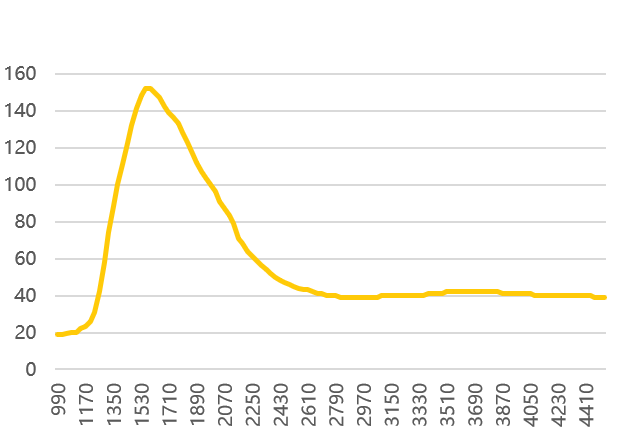
\includegraphics[width=0.7\linewidth]{图片2.png}
	\caption{The flow curve of Sephadex Gel G100 Filtration (5ml/min)}
	\label{fig:g1001}
\end{figure}

\begin{figure}[!h]
	\centering
	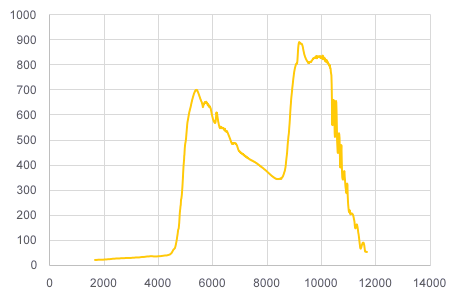
\includegraphics[width=0.7\linewidth]{图片1.png}
	\caption{The flow curve of Sephadex Gel G100 Filtration (0.5ml/min), absorbance versus second}
	\label{fig:g1002}
\end{figure}

\subsection{Verification through SDS-PAGE}

The first SDS-PAGE was introduced after the \emph{G-100 Sephadex} size
exclusion chromatography. The result is listed as follows. There are
five different swim lanes from A1 to A5 in the graph, constructing a
concentration gradient. The chromatography shows that the main products
extracted from the solution located at 40-70 kDa while only little
product locates at \textasciitilde{}10 kDa, where lysozyme will be. We refer to the article to find out the reasons that may lead to the phenomena and find that the chromatography distribution of our examples is similar to the natural distribution of proteins in
eggs.

\begin{figure}[!h]
	\centering
	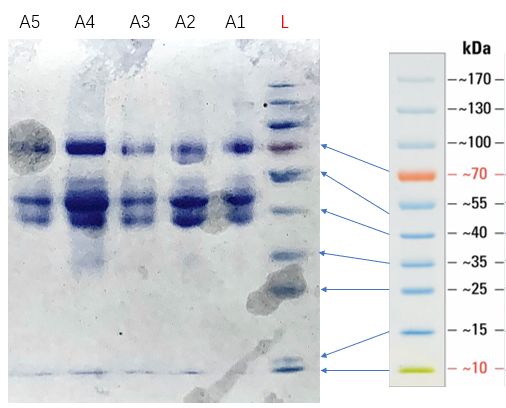
\includegraphics[width=0.7\linewidth]{图片3.png}
	\caption{Electrophoresis results of Sephadex Gel G100 Filtration (compared with \citet{Liu2020})}
	\label{fig:g100}
\end{figure}

These facts convince us of the experimental failure and difficulties
using size exclusion chromatography to extract the lysozyme. Hence we
purchase the \emph{732 cation exchange resin} to conduct the further
experiment.

\section{Cation Exchange with Resin 732}

\subsection{Results}
We repeated this experiment on both a small column and a much bigger one. For simplicity, we abbrivate "concentrated elution peak from bigger column" to EPB and "concentrated elution peak from smaller column" to EPS.

During the elution, both of the scenerios showed only one peak.

\subsection{Verification through SDS-PAGE}

We made our second SDS-PAGE after the liquid chromatography and get really exciting results. There are three swim lanes in this PAGE-B1, B2 and B3. B2 is the commercial lysozyme product (2g/L) which we bought to examine the
resin as a standard product. B1,B3 is the concentrated solution extracted by the small column and big column, respectively. According to the result, all the examples located around
the 10-15kDa site, indicating the existence of lysozyme. \textbf{There is almost no other bands, indicating the thrilling purity of lysozyme.} We also notice
that the abundance of B1 and B3 are similar, which means the inspiring concentration of our extracted lysozyme.

\begin{figure}[!h]
	\centering
	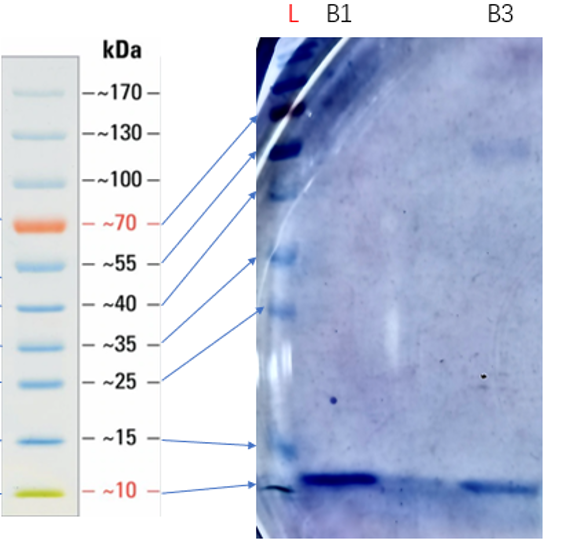
\includegraphics[width=0.7\linewidth]{图片4.png}
	\caption{Electrophoresis results of Resin 732 Cation Exchange}
\end{figure}

\subsection{Summary on Two Types of Separation Methods}
\begin{figure}[!h]
	\centering
	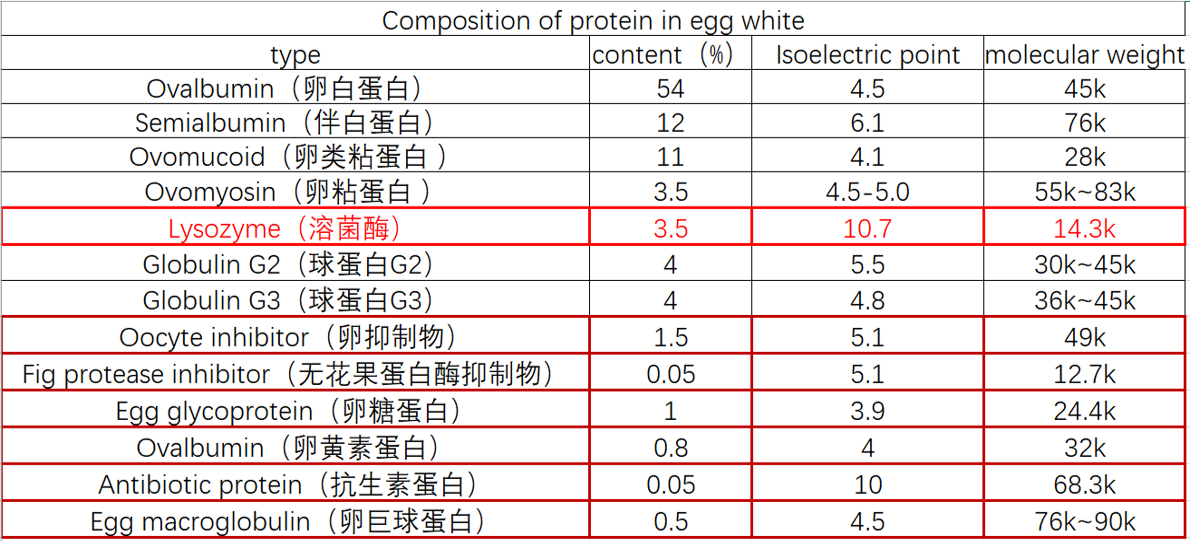
\includegraphics[width=0.7\linewidth]{lyso.png}
	\caption{Composition of proteins in egg white \citep{Zhang2003}}
	\label{tab:compo}
\end{figure}

According to this chart (Fig. \ref{tab:compo}), we once believed that separation according to molecular weight might be successful. However, the first experimental design failed. The reason may be: the column is not long enough to separate all composites. We think the flow rate at 0.5 mL/min is not worthy to be decreased further, and no other factors matter if we don't change the filler. On the other side, Resin 732 helped us succeed because there is nearly no impurities at isoelectric point of more than 10 (the content of antibiotic protein is so low as to be ignored).


\section{Effect of pH on Enzyme Activity}

The absorbance curves, which were measured under identical condition, are shown in Fig \ref{fig:ph} and \ref{fig:ph89}. 
\begin{figure}[!h]
	\centering
	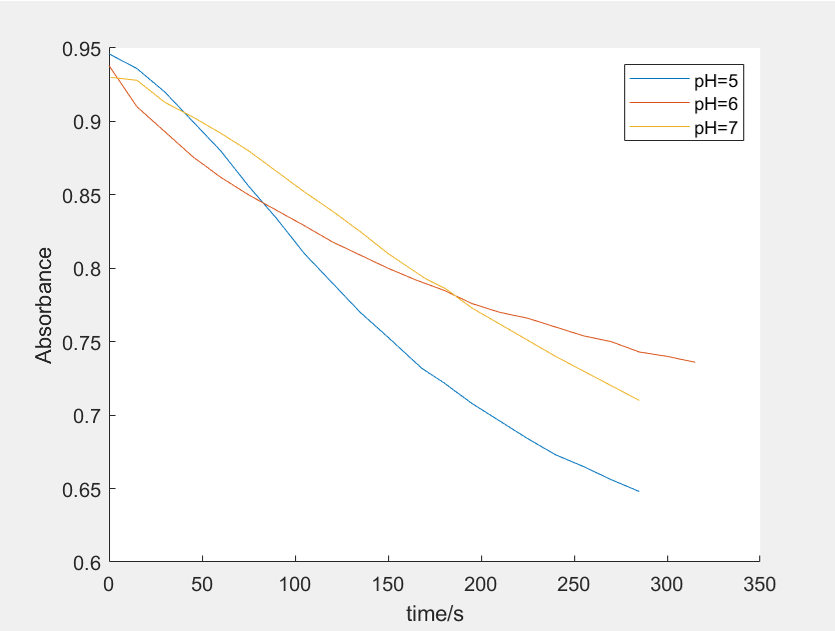
\includegraphics[width=0.9\linewidth]{figures/chp3_ph}
	\caption{Absorbance curves (pH=5,6,7)}
	\label{fig:ph}
\end{figure}

\begin{figure}[!h]
	\centering
	\begin{minipage}[c]{0.45\textwidth}
		\centering
		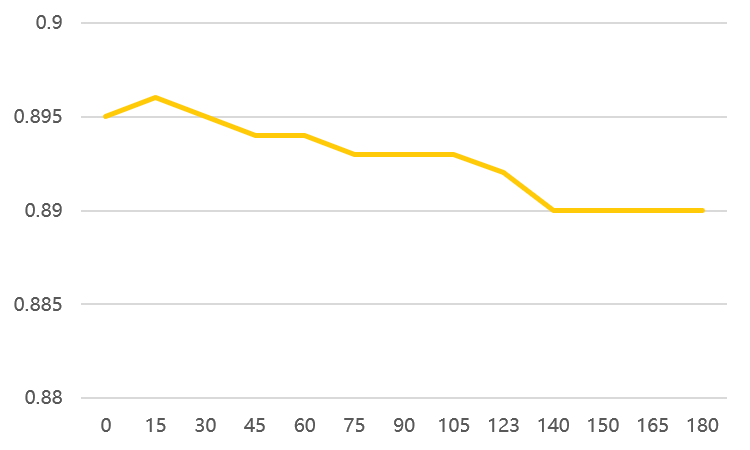
\includegraphics[width=\linewidth]{chp3_ph8}
	\end{minipage}
	\quad
	\begin{minipage}[c]{0.45\textwidth}
		\centering
		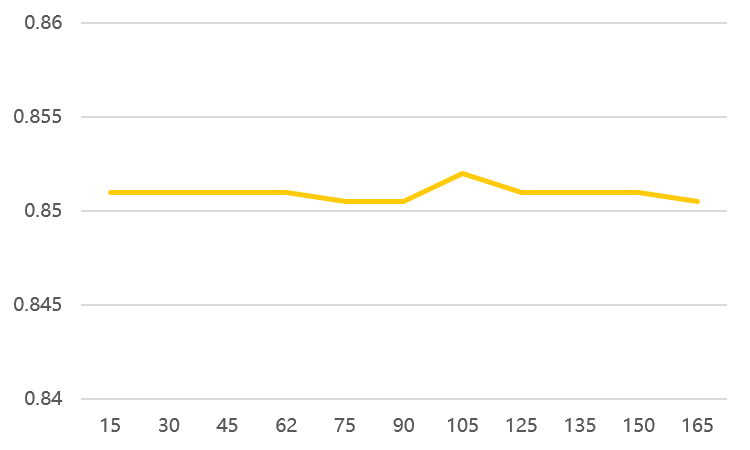
\includegraphics[width=\linewidth]{chp3_ph9}
	\end{minipage}
	\caption{Absorbance curves (pH=8,9)}
	\label{fig:ph89}
\end{figure}


Obviously, the lysozyme almost lose all its activity under pH 8 and 9. For the other three groups, we can roughly believe that the enzyme activity is highest when pH=5. However, we found in plenty of literature \citep{Yu-tong2006,Tian2012} that the optimal pH of lyzozyme is about 6. We also refered to some other groups of experiments, and found activity of lyzozyme when pH=6 is similar. 

This suggests that there might be some problem with the buffer (pH=6). Perhaps one of the reasons is that the pH test paper we used has low accuracy. Another problem is that enzyme activity should not be so low at pH 8 and 9. pH of egg white is about 8.0 and we used buffer whose pH is 9.0 to elute lysozyme from our column. Perhaps there is a shift in pH towards higher values when we were testing the activity, which could explain the optimal pH (5) might be larger and the activity problem. But this is not so possible. We believe we did not make such mistakes when configuring the buffers.

Unfortunately, we did not discover this fact at the time of experiment. So we go on to test enzyme activity when pH is tagged 6 (but may be 7 actually), which the literature indicated as an optimum.

\section{Enzyme Activity Calculation}

\begin{figure}[!h]
	\centering
	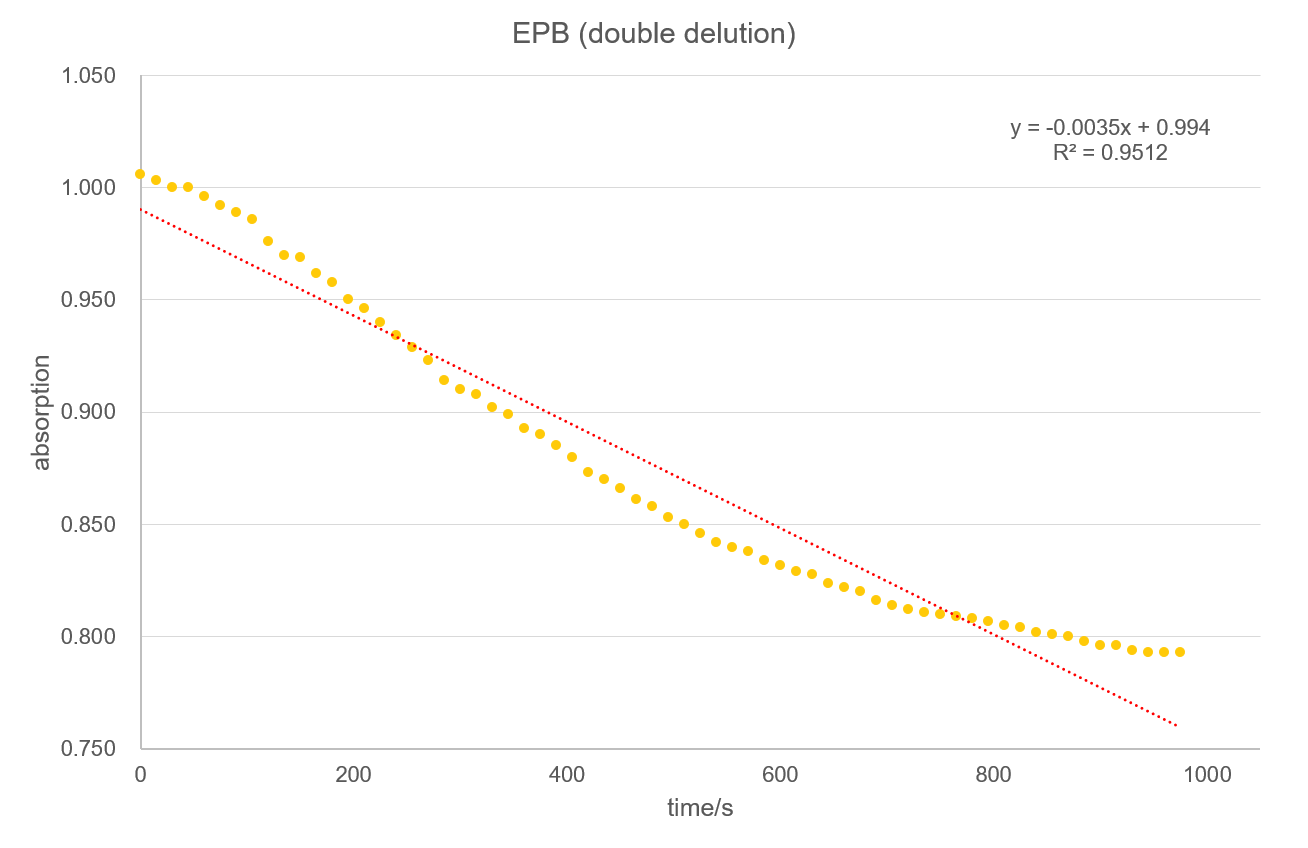
\includegraphics[width=0.9\linewidth]{figures/chp3_EPBcur}
	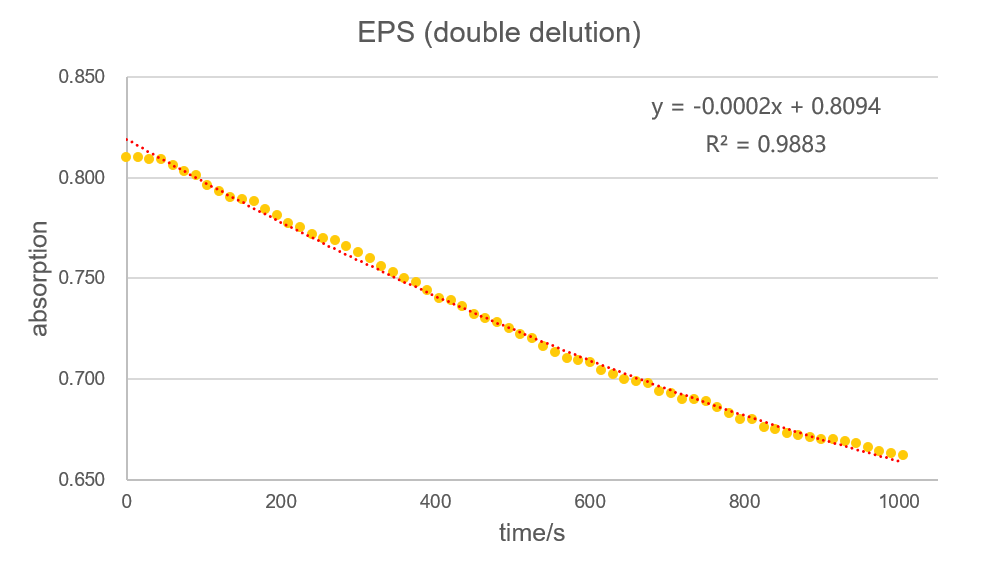
\includegraphics[width=0.9\linewidth]{figures/chp3_EPScur}
	\caption{Enzyme activity of the elution peaks}
	\label{fig:epbs}
\end{figure}

%\begin{figure}[!h]
%	\centering
%	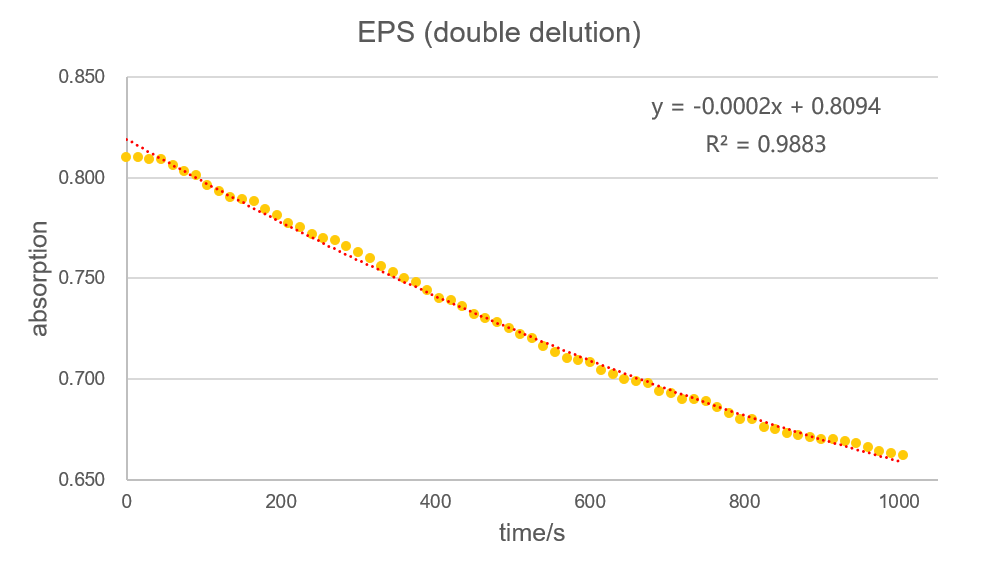
\includegraphics[width=0.7\linewidth]{figures/chp3_EPScur}
%	\caption{a skecth of our polygon-sphere}
%	\label{fig:eps}
%\end{figure}

According to the definition mentioned in Sec. 2, we can calculate the enzyme activity of the concentrated solutions. We picked a linear region on the whole curve (See Fig \ref{fig:epbs}). The first few data points should be avoided because the mixture hasn't become homogenous and the reaction hasn't reached a steady state. We actually picked the 2nd minute, which means
\begin{gather*}
	EnzymeActivity=\dfrac{OD_{600}(120\mathrm{s})-OD_{600}(60\mathrm{s})}{0.5\mathrm{mL}}\times 10^{3}
\end{gather*}

The concentration we directly measured by the instrument is listed in Tab. \ref{tab:conc}:
\begin{table}[!h]
	\centering
	\caption{Concentration of concentrated enzyme solutions}
	\begin{tabular}{ccc}
		\toprule
		& {EPB (double dilution)} & {EPS EnzymeActivity} \\
		\midrule
		concentration $(\mathrm{g\cdot L^{-1}})$ & $3.725$  & $2.832$ \\
		\bottomrule
	\end{tabular}%
	\label{tab:conc}%
\end{table}%
which shows EPB was concentrated more times than EPS.

The activity results are listed in Tab. \ref{tab:res}:
\begin{table}[!h]
	\centering
	\caption{Enzyme Activity}
	\begin{tabular}{ccc}
		\toprule
		& {EPB (double dilution)} & {EPS (double dilution)} \\
		\midrule
		EnzymeActivity $(\mathrm{U\cdot mL^{-1}})$ & $50.0$  & $32.5$ \\
		SpecificActivity $(\mathrm{U\cdot mg^{-1}})$ & $13.4$ & $11.5$\\
		\bottomrule
	\end{tabular}%
	\label{tab:res}%
\end{table}%

Enzyme activities are of the same order of magnitude as that in the literature. 
There is no significant difference between the specific activities, which is a rational result.

Moreever, we also calculated the recovery rate of the bigger column roughly, but we did not record the exact loading volume.

\begin{table}[!h]
	\centering
	\caption{Recovery rate}
	\begin{tabular}{cc}
		\toprule
		& {EPB (double dilution)}\\
		\midrule
		Approximate loading volume/mL  & $6.5$ \\
		Recovery rate  & $92.4\%$ \\
		\bottomrule
	\end{tabular}%
	\label{tab:rec}%
\end{table}%

The result is also fascinating, which is probably due to a properly chosen elution pH.

\section{Reaction Kinetics Exploration}

In the previous sections, we have treated the absorbance curves as linear. But all curves seem to to plain as time passes, which means the reaction rate is decreasing slightly. As we used 2g/L standard enzyme when exploring the effect of pH, we believe it is likely that Machaelis-Menten equation doesn't apply here due to lower and lower substrate (bacteria) concentration. To better and fully describe the reaction, and to find indexes to measure enzyme activity without the influence of reactant concentrations, we explored the reaction kinetics.

We assume that substrate concentration is proportional to the absorbance, and tried many functions, and the results are listed in Tab \ref{tab:fit}. All are performed in Excel and MATLAB. Below the third horizontal line, there are several functions for which I cannot find actual meanings.

\begin{table}[!h]
	\centering
	\caption{Results of Fit}
	\begin{tabular}{ccccc}
		\toprule
		function & expression and data & pH=5 & pH=6 & pH=7 \\
		\midrule
		linear & $at+b$; 0-order reaction & 0.9717  & 0.9871  & 0.9667  \\
		MM as rate & $\int \mathrm{d}c/\mathrm{d}t=v\cdot c/(c+k_s)$ & unrational & unrational & 0.9944  \\
		MM as rate & same but without the first three points & 0.9574  & 0.9665  & 0.9545  \\
		MM as rate & $\int \mathrm{d}c/\mathrm{d}t=v\cdot c^2/(c+k_s)$ & 0.9842  & unrational & unrational \\
		exponential & $a\cdot \exp(bt)$; 1-order reaction & 0.9848  & 0.9791  & 0.9869  \\
		\midrule
		polynomial & $at^2+bt+c$ & 0.9968  & 0.9972  & 0.9981  \\
		\textbf{polynomial} & same but without the first three points & \textbf{0.9994}  & \textbf{0.9993}  & \textbf{0.9994} \\
		rational & $a/(t+b)$ & 0.9942  & 0.9961  & 0.9952  \\
		rational & $a/(t+b)+c$ & 0.9968  & 0.9965  & 0.9973  \\
		logistic & $a/(1+b\cdot \exp(ct))$ & 0.9832  & 0.9549  & 0.9840  \\
		\bottomrule
	\end{tabular}%
	\label{tab:fit}%
\end{table}%

We can see that:
\begin{itemize}
	\item
	Linear functions, which means the rate is constant, don't fit very
	well. Exponetial functions which imply the rate is proportional to
	substrate concentration, fit a bit better.
	\item
	If the rate complies with MM equation
	\[\dfrac{\mathrm{d}c}{\mathrm{d}t}=-v_m\cdot c/(c+k_s)\]
	we integrated it and failed to drive a meaningful result, because
	either \(R^2\) is low or \(K_s\) is negative or unrationally large.
	\item
	We also assume that when enzyme concentration is large, only part of
	the enzyme molecules bind to the substrate. The "effective" enzyme
	concentration is proportional to the substrate concentration. This can
	also be verified by modifying the derivation of MM equation. Thus
	\[\dfrac{\mathrm{d}c}{\mathrm{d}t}=-k_{cat}\cdot c^2/(c+k_s)\]
	However, this also failed because \(K_s\) is negative or too large,
	which leads that lower substrate concentration makes higher rate.
	\item
	The last three fits are just based on similar curve shape. We cannot
	explain them.
\end{itemize}

The most interesting one is polynomial fit, which fits best.
Especially when we delete the first three "unsteady-state" data points. However, it doesn't make sense. It is strange to have an chemical equation whose rate is proportional to reaction time. The integral of MM equation is a implicit function, so we don't have access to the terms and their meanings. This might be a problem waiting for mathematicians and chemists to solve.

The most rational explanation is, this quadratic function is a Taylor expansion (\eqref{tay}) of a more complex function or model that we haven't found out. 
\begin{equation}
	f(x)=f(x_0)+\dfrac{f^{\prime}(x_0)}{1!}(x-x_0)+\dfrac{f^{\prime \prime}(x_0)}{2!}(x-x_0)^2+\cdots \label{tay}
\end{equation}

We may divide $c_s=at^2+bt+c$ into:
\begin{itemize}
	\item constant $c$;
	\item linear part $bt$, which correspond to constant-rate reaction, like the early state of MM enzymatic reaction;
	\item nonlinear part $at^2$, which is the bias caused by some factors.
\end{itemize}

We think that $b$ decides the rate, or the enzyme activity. 

\begin{table}[!h]
	\centering
	\caption{Polynomial fit parameters}
	\begin{tabular}{cccc}
		\toprule
		parameters & pH=5  & pH=6  & pH=7 \\
		\midrule
		a     & 2.46e-06 & 1.20e-06 & 9.00e-07 \\
		b     & -1.86e-03 & -9.49e-04 & -1.10e-03 \\
		c     & 0.9788 & 0.9163 & 0.9537 \\
		\bottomrule
	\end{tabular}%
	\label{tab:para}%
\end{table}%

The results are not ideal too due to the pH problem. However, we propose this model to understand a nonlinear biological reaction curve like this. By analyzing the both parts, we may gain information about enzyme activity, reaction type, etc.



        % multiple1902 <multiple1902@gmail.com>
% conclusion.tex
% Copyright 2011~2012, multiple1902 (Weisi Dai)
% https://code.google.com/p/xjtuthesis/
% 
% It is strongly recommended that you read documentations located at
%   http://code.google.com/p/xjtuthesis/wiki/Landing?tm=6
% in advance of your compilation if you have not read them before.
%
% This work may be distributed and/or modified under the
% conditions of the LaTeX Project Public License, either version 1.3
% of this license or (at your option) any later version.
% The latest version of this license is in
%   http://www.latex-project.org/lppl.txt
% and version 1.3 or later is part of all distributions of LaTeX
% version 2005/12/01 or later.
%
% This work has the LPPL maintenance status `maintained'.
% 
% The Current Maintainer of this work is Weisi Dai.
%

\chapter{结论与展望}
%
%    \xjtuthesis 是一个开源项目,旨在提供符合西安交通大学有关部门要求的学位论文\LaTeX 模板。
%
%    您当前看到的文件是 \xjtuthesis{} \metaversion 的示例排版文档。
%
%    \xjtuthesis 项目目前托管在Google Code: \verb|http://xjtuthesis.googlecode.com/|
%    
%    \xjtuthesis 采用Mercurial管理源代码。访问项目的网站,了解更多信息。
%
%    \section{使用\xjtuthesis}
%
%        如果你是本科生,请和系里联系以确定可以使用\xjtuthesis 完成论文。
%
%        研究生请和西安交大研究生院学位办(周主任)联系:
%        
%        \begin{description}
%            \item[电话] 82668899
%            \item[办公地址] 教学主楼1311室
%            \item[电子邮件] \url{xwb@mail.xjtu.edu.cn} (从来不回)
%        \end{description}


%        % multiple1902 <multiple1902@gmail.com>
% float.tex
% Copyright 2011~2012, multiple1902 (Weisi Dai)
% https://code.google.com/p/xjtuthesis/
% 
% It is strongly recommended that you read documentations located at
%   http://code.google.com/p/xjtuthesis/wiki/Landing?tm=6
% in advance of your compilation if you have not read them before.
%
% This work may be distributed and/or modified under the
% conditions of the LaTeX Project Public License, either version 1.3
% of this license or (at your option) any later version.
% The latest version of this license is in
%   http://www.latex-project.org/lppl.txt
% and version 1.3 or later is part of all distributions of LaTeX
% version 2005/12/01 or later.
%
% This work has the LPPL maintenance status `maintained'.
% 
% The Current Maintainer of this work is Weisi Dai.
%
\chapter{浮动格式}

    金溪民方仲永,世隶耕。仲永生五年,未尝识书具,忽啼求之。父异焉,借旁近与之,即书诗四句,并自为其名。其诗以养父母、收族为意,传一乡秀才观之。自是指物作诗立就,其文理皆有可观者。邑人奇之,稍稍宾客其父,或以钱币乞之。父利其然也,日扳仲永环谒于邑人,不使学。

    余闻之也久。明道中,从先人还家,于舅家见之,十二三矣。令作诗,不能称前时之闻。又七年,还自扬州,复到舅家问焉。曰:“泯然众人矣。”

    王子曰:仲永之通悟,受之天也。其受之天也,贤于才人远矣。卒之为众人,则其受于人者不至也。彼其受之天也,如此其贤也,不受之人,且为众人;今夫不受之天,固众人,又不受之人,得为众人而已耶?

    \section{图片}

        \begin{figure}[h!]
          \centering
          
\includegraphics[width=6.67cm]{XJTU.pdf}
          \caption{西安交通大学}
          \label{fig:xjtu}
        \end{figure}

        \begin{figure}[h!]
          \begin{minipage}{0.45\textwidth}
              \centering
              
\includegraphics[width=6.67cm]{XJTU.pdf}
              \caption{西安交通大学}
              \label{fig:xjtu-left}
          \end{minipage}
          \begin{minipage}{0.45\textwidth}
              \centering
              
\includegraphics[width=6.67cm]{XJTU.pdf}
              \caption{西安交通大学}
              \label{fig:xjtu-right}
          \end{minipage}
        \end{figure}
          
        \begin{figure}[h!]
          \centering
          \subfloat[果毅力行]{
              
\includegraphics[width=6.67cm]{XJTU.pdf}
              \label{fig:xjtu-sub-left}}
          \subfloat[忠恕任事]{
              
\includegraphics[width=6.67cm]{XJTU.pdf}
              \label{fig:xjtu-sub-right}}
          \caption{子图}
        \end{figure}
          

    \section{表格}

        \begin{table}[h!]
          \centering
          \caption{一个简单的表格}
          \label{tab:simple}
          \wuhao
          \begin{tabularx}{\linewidth}{XXXXX} \toprule 
                & 一月 & 二月 & 三月 & 合计 \\ \midrule
           东部 &    7 &    7 &    5 &   19 \\ 
           西部 &    6 &    4 &    7 &   17 \\ 
           南部 &    8 &    7 &    9 &   24 \\ 
       \bf 合计 &   21 &   18 &   21 &   60 \\ \bottomrule
          \end{tabularx}
        \end{table}


        \begin{table}[h!]
          %\begin{minipage}{\textwidth}
          \begin{threeparttable}[h]
            \centering
            \caption{包含脚注的表格}
            \label{tab:with-footnote}
            \wuhao
            \begin{tabularx}{\linewidth}{XXXXX} \toprule 
                  & 一月 & 二月 & 三月 & 合计 \\ \midrule
                  东部 &    7\tnote{1}
                                &    7 &    5 &   19 \\ 
             西部 &    6 &    4 &    7 &   17 \\ 
             南部 &    8 &    7 &    9 &   24 \\ 
             \bf 合计\tnote{2}
                  &   21 &   18 &   21 &   60 \\ \bottomrule
            \end{tabularx}
          %\end{minipage}
          \begin{tablenotes}
          \item[1] 数据来自Word 97.
          \item[2] Computed by \textsl{Mathematica} 8.
          \end{tablenotes}
          \end{threeparttable}
        \end{table}

        \begin{table}[h!]
          \centering
          \caption{稍微复杂一点的表格}
          \label{tab:complex}
          \wuhao
          \begin{tabularx}{\linewidth}{XXXXX} \toprule 
                & \multicolumn{3}{c}{这是一句废话} &  \\ \cmidrule{2-4}
                & 一月 & 二月 & 三月 & 合计 \\ \midrule
           东部 &    7 &    7 &    5 &   19 \\ 
           西部 &    6 &    4 &    7 &   17 \\ 
           南部 &    8 &    7 &    9 &   24 \\ 
       \bf 合计 &   21 &   18 &   21 &   60 \\ \bottomrule
          \end{tabularx}
        \end{table}

        我制作了一个简单的表格(表\ref{tab:simple})。


%        % multiple1902 <multiple1902@gmail.com>
% formulae.tex
% Copyright 2011~2012, multiple1902 (Weisi Dai)
% https://code.google.com/p/xjtuthesis/
% 
% It is strongly recommended that you read documentations located at
%   http://code.google.com/p/xjtuthesis/wiki/Landing?tm=6
% in advance of your compilation if you have not read them before.
%
% This work may be distributed and/or modified under the
% conditions of the LaTeX Project Public License, either version 1.3
% of this license or (at your option) any later version.
% The latest version of this license is in
%   http://www.latex-project.org/lppl.txt
% and version 1.3 or later is part of all distributions of LaTeX
% version 2005/12/01 or later.
%
% This work has the LPPL maintenance status `maintained'.
% 
% The Current Maintainer of this work is Weisi Dai.
%
\chapter{公式环境}

    \begin{axiom}
        \rm 两点间直线段距离最短。  
        \begin{align}
            x&\equiv y+1\pmod{m^2}\\
            x&\equiv y+1\mod{m^2}\\
            x&\equiv y+1\pod{m^2}
        \end{align}
    \end{axiom}

    \begin{remark}
    \rm 对齐的公式示例,它还同时演示了标号。
    \begin{align}
    \begin{split} 
    \varphi(x,z)
    &=z-\gamma_{10}x-\gamma_{mn}x^mz^n\\
    &=z-Mr^{-1}x-Mr^{-(m+n)}x^mz^n
    \end{split} \notag \\
    \noindent\zeta^1&=(\xi^1)^2,\\
    \zeta^1 &=\xi^0\xi^1,\\
    \zeta^2 &=(\xi^1)^2,
    \end{align}
    \end{remark}

    \begin{theorem}
      \rm 对于直角三角形$ABC$, 若$a<c$且$b<c$, 则有
        \begin{equation}
          a^2+b^2=c^2
        \end{equation}
    \end{theorem}


    \begin{exercise}
          \rm 请列出温家宝的所有影视作品。
    \end{exercise}
        
    贝叶斯公式如式~(\ref{equ:chap1:bayes}),其中 $p(y|\mathbf{x})$ 为后验;
    $p(\mathbf{x})$ 为先验;分母 $p(\mathbf{x})$ 为归一化因子。
    \begin{equation}
        \label{equ:chap1:bayes}
        p(y|\mathbf{x}) = \frac{p(\mathbf{x},y)}{p(\mathbf{x})}=
        \frac{p(\mathbf{x}|y)p(y)}{p(\mathbf{x})} 
    \end{equation}


    \xjtuendcontent

%    \xjtubib{references}	
	\bibliography{references}

%    \xjtuappendix

%        % multiple1902 <multiple1902@gmail.com>
% appendice.tex
% Copyright 2011~2012, multiple1902 (Weisi Dai)
% https://code.google.com/p/xjtuthesis/
% 
% It is strongly recommended that you read documentations located at
%   http://code.google.com/p/xjtuthesis/wiki/Landing?tm=6
% in advance of your compilation if you have not read them before.
%
% This work may be distributed and/or modified under the
% conditions of the LaTeX Project Public License, either version 1.3
% of this license or (at your option) any later version.
% The latest version of this license is in
%   http://www.latex-project.org/lppl.txt
% and version 1.3 or later is part of all distributions of LaTeX
% version 2005/12/01 or later.
%
% This work has the LPPL maintenance status `maintained'.
% 
% The Current Maintainer of this work is Weisi Dai.
%
\xjtuappendixchapter{附录}

    \xjtuappendixsection{测试标题}

        The quick brown fox jumps over the lazy dog.

        \begin{figure}[h!]
          \centering
          
\includegraphics[width=6.67cm]{XJTU.pdf}
          \caption{西安交通大学}
          \label{fig:in-appendix}
        \end{figure}

        \xjtuappendixsubsection{三级标题}

            测试

            \xjtuappendixsubsubsection{四级标题}

                测试

\xjtuappendixchapter{还是附录}

    \xjtuappendixsection{测试}

        The quick brown fox jumps over the lazy dog.


%    \xjtuendappendix

    \xjtuspchapter{致谢}{致\qquad 谢} % 致\qquad 谢

        
谨此向孔宇教授致以衷心的感谢和崇高的敬意!



%美哉吾校, 真理之花, 青年之模楷, 邦国之荣华, 
%
%校旗飘扬, 与日俱长, 为世界之光, 为世界之光. 
%
%美哉吾校, 鼓舞群伦, 启发我睿智, 激励我热忱, 
%
%英俊济跄, 经营四方, 为世界之光, 为世界之光. 
%
%美哉吾校, 性灵泉源, 科学之奥府, 艺术之林园, 
%
%实业扩张, 进步无疆, 为世界之光, 为世界之光. 
%
%美哉吾校, 灿烂文明, 实学培国本, 民族得中兴, 
%
%宇土茫茫, 山高水长, 为世界之光, 为世界之光. 


\end{document}

